\documentclass[12pt]{article}
\usepackage{scribe}

\Scribe{Ryan O'Donnell}
\Lecturer{Ryan O'Donnell}
\LectureNumber{1}
\LectureDate{September 9, 2015}
\LectureTitle{Introduction to the Quantum Circuit Model}

% macros local to this lecture
\newcommand{\COIN}{\mathrm{COIN}}
\newcommand{\CCOIN}{\mathrm{CCOIN}}

\begin{document}

\MakeScribeTop

\section{Overview of what is to come}

\subsection{An incredibly brief history of quantum computation}

The idea of quantum computation was pioneered in the 1980s mainly by Feynman~\cite{Fey82,Fey86} and Deutsch~\cite{Deu85,Deu89}, with Albert~\cite{Alb83} independently introducing quantum automata and with Benioff~\cite{Ben80} analyzing the link between quantum mechanics and reversible classical computation.  The initial idea of Feynman was the following: Although it is perfectly possible to use a (normal) computer to simulate the behavior of $n$-particle systems evolving according to the laws of quantum, it seems be extremely inefficient.  In particular, it seems to take an amount of time/space that is exponential in~$n$.  This is peculiar because the actual particles can be viewed as simulating \emph{themselves} efficiently. So why not call the particles themselves a ``computer''?  After all, although we have sophisticated theoretical models of (normal) computation, in the end computers are ultimately physical objects operating according to the laws of physics.  If we simply regard the particles following their natural quantum-mechanical behavior as a computer, then this ``quantum computer'' appears to be performing a certain computation (namely, simulating a quantum system) exponentially more efficiently than we know how to perform it with a normal, ``classical'' computer.  Perhaps we can carefully engineer multi-particle systems in such a way that their natural quantum behavior will do \emph{other} interesting computations exponentially more efficiently than classical computers can.

This is the basic idea behind quantum computers.  As it turns out, you \emph{can} get (seemingly) exponential speedups for a (seemingly) small number of natural computational problems by carefully designing a multi-particle quantum system and letting it evolve according to the (100-year old, extremely well-confirmed) laws of quantum mechanics.  By far the most spectacular example is Shor's factoring algorithm~\cite{Sho97}, an algorithm implementable on a quantum computer that can factor any $n$-digit integer (with high probability) in roughly~$n^2$ time.  This is contrast to the fact that the fastest known ``classical'' algorithm for factoring $n$-digit integers seems to require roughly $2^{n^{1/3}}$ time, and in fact the presumed computational difficulty of factoring is relied upon in an enormous number of real-world cryptographic applications (e.g., the computations done whenever you type \texttt{https://} into your browser).

\subsection{Plans for this course and this lecture}

Very briefly, in this course we will:
\begin{itemize}
    \item \emph{Mathematically} formulate the tiny bit of quantum mechanics that is relevant for the field of quantum computation.  (We should mention that this course will be heavily slanted towards theoretical computer science and mathematics, and will contain almost no physics.)
    \item See some quantum algorithms that solve certain computational problems much faster than they are known to be solvable classically.
    \item Investigate the \emph{limits} of quantum computation.  (It is \emph{not} the case that quantum computation automatically provides speedup over classical computation for all problems, or even for a wide class of problems.)
    \item Study some quantum information theory.
\end{itemize}

The goal for this first lecture is to give a lightning-fast, as-barebones-as-possible definition of the quantum circuit model of computation.  After this lecture, you will theoretically know all you need to know in order to implement and analyze, e.g., Shor's algorithm.  (Of course, we will subsequently make a more thorough and leisurely development of quantum computation before actually getting around to sophisticated algorithms.)

$90\%$ of the understanding of the quantum circuit model is achieved by reviewing three purely ``classical'' topics: classical Boolean circuits; reversible classical circuits; and randomized computation.  The first and third of these topics should be very familiar to anyone who has studied the basics of theoretical computer science.  And the second topic is very cute and elementary. Once we have these three concepts in hand, quantum circuits become practically just a tiny ``twist'' on randomized computation --- what you might get if you tried to invent a model of randomized computation in which ``probabilities'' can be \emph{negative}\dots

\section{Classical Boolean circuits}

Several models of computation/algorithms are studied in the classical theory of computation: Turing Machines, high-level programming languages, and Boolean circuits.  It turns out that for the study of quantum computation, the Boolean circuit model is by far the easiest model to generalize (being as it the closest model of the physical reality of computers).

We begin with the following well known fact, stating that any computational task (modeled by a Boolean function) we might want to do is doable with an $\AND$/$\OR$/$\NOT$ Boolean circuit.
\begin{proposition}                                     \label{prop:universal1}
    Any Boolean function $f : \{0,1\}^n \to \{0,1\}^m$ is computable by a Boolean circuit $C$ using just $\AND$, $\OR$, and $\NOT$ gates. I.e., $\AND$, $\OR$, and $\NOT$ gates are \emph{universal}.
\end{proposition}
\begin{remark}
    The $\AND$ and $\OR$ gates mentioned in this proposition take $2$ input bits and produce $1$ output bit.  The $\NOT$ gate takes $1$ input bit and produces $1$ output bit.
\end{remark}
\begin{remark}
    Once we know that every Boolean function is computable by some circuit, we usually become interested in computing it \emph{efficiently}; i.e., with a circuit~$C$ of small \emph{size}.  The size of the circuit, $\size(C)$, is defined to be the number of gates it uses. Circuit size fairly closely corresponds to \emph{running time} in the Turing Machine (sequential algorithm) model.  For example, it is known that a circuit of size $s$ can be evaluated in time $O(s \log s)$ by a Turing Machine, and conversely, a Turing Machine operating in time~$t$ on length-$n$ inputs can be converted to an $n$-input circuit of size $O(t \log t)$.
\end{remark}

Here is a simple example of a circuit computing the $\XOR$ function, $f(x_1, x_2) = x_1 \oplus x_2$:
\begin{center}
        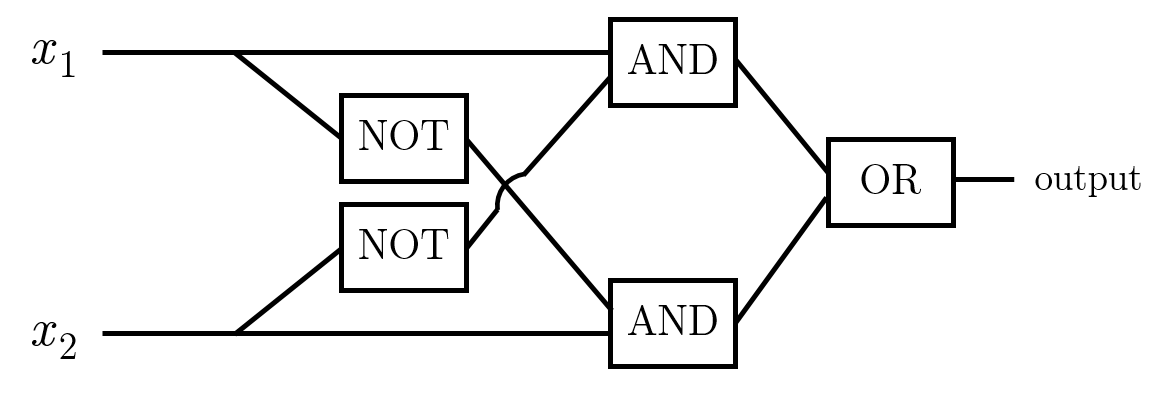
\includegraphics[scale=.5]{lecture01-figure1.png}
\end{center}
The lines in this diagram are called ``wires'', and the things inside the rectangles are called ``gates''.  In the diagram we have followed a traditional circuit-theory convention by allowing wires to ``branch''; i.e., split into two copies.  In reality, some physical mechanism must exist at these branches, and in the future it will be convenient to make this explicit.  So we will introduce a new kind of gate called a $\DUPE$ (\emph{duplicate}) gate which takes $1$ input bit and outputs $2$ duplicate copies of that bit.  We will then redraw the above diagram as follows:
\begin{center}
        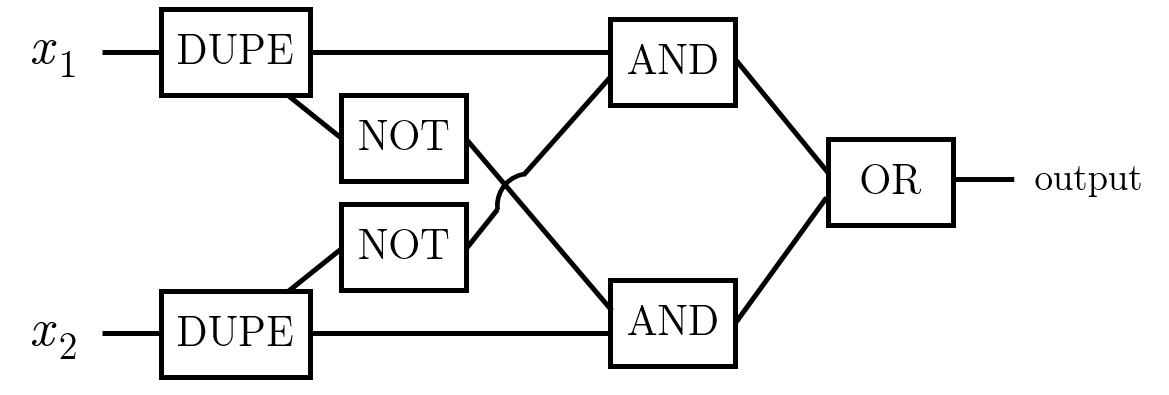
\includegraphics[scale=.5]{lecture01-figure2.png}
\end{center}
With this convention, it would be more accurate to say that $\AND$, $\OR$, $\NOT$, and $\DUPE$ gates are universal for Boolean circuit computation.

It is also a well known fact that one can get smaller universal gate sets; in fact, one can replace $\AND$/$\OR$/$\NOT$ gates with just NAND gates.  (Recall that $\NAND(x_1,x_2) = \NOT(\AND(x_1,x_2))$.)  To see this, first note that we can eliminate $\OR$ gates using De~Morgan's rule: $\OR(x_1, x_2) = \NOT(\AND(\NOT(x_1),\NOT(x_2)))$. Then we can eliminate $\AND$ gates in favor of $\NAND$ gates via $\AND(x_1,x_2) = \NOT(\NAND(x_1, x_2))$.  Finally, we need to show that $\NOT$ gates can be eliminated using $\NAND$ gates.  One way to implement $\NOT(x_1)$ with a $\NAND$ gate is as follows:
\begin{center}
        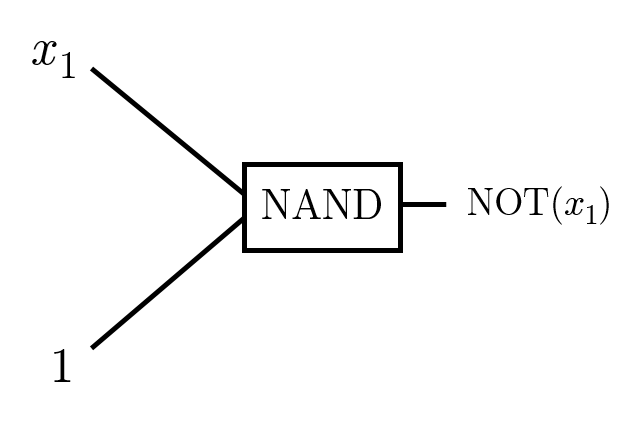
\includegraphics[scale=.5]{lecture01-figure3.png}
\end{center}
On the lower left in this diagram, we have what is called an \emph{ancilla} bit: an input that is ``hardwired'' to the constant bit~$1$, for the purposes of assisting the computation.  It's actually possible to implement $\NOT(x_1)$ using $\NAND$ and $\DUPE$ without the use of ancillas (specifically, via $\NAND(\DUPE(x_1))$).  However the above method gives us a good opportunity to introduce the notion of ancillas.

What we have just shown is the following:
\begin{proposition}                                     \label{prop:universal2}
    Boolean $\NAND$ and $\DUPE$ gates (along with the use of ancillas) are \emph{universal} for computation.
\end{proposition}
\begin{remark}
    In fact, we have shown something stronger: Not only can every $\AND$/$\OR$/$\NOT$/$\DUPE$ circuit $C$ be converted to an equivalent $\AND$/$\OR$/$\NOT$ circuit~$C$', this conversion can be done very \emph{efficiently}; there is an efficient algorithm carrying out the conversion, and $\size(C') = O(\size(C))$.
\end{remark}

\subsection{Bra-ket notation}

We take this opportunity to introduce a bit of unusual notation that will play an essential role in the remainder of the course.  This is the ``bra-ket'' notation invented by Paul Dirac.  Actually, we will postpone the mathematical definitions to the next lecture; for now we will just introduce it as pure symbolism.  We will henceforth enclose bits and bit-strings in asymmetrical brackets called \emph{kets}, writing $\ket{0}$ and $\ket{1}$ instead of $0$ and $1$.  We will also usually eliminate internal brackets when writing strings; e.g., writing $\ket{011}$ instead of $\ket{0}\ket{1}\ket{1}$.  As a small example of this notation, we will redraw the previous diagram as follows:
\begin{center}
        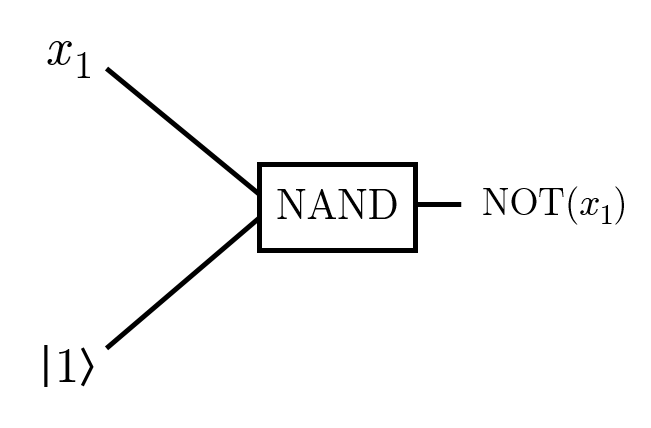
\includegraphics[scale=.5]{lecture01-figure4.png}
\end{center}


\section{Reversible computation}

In actual physical reality, a theoretical bit ($\ket{0}$ or $\ket{1}$) is implemented by a particle or bunch of particles (e.g., high or low voltage on a physical wire).  Similarly, a gate is implemented by a physical object (a ``switch'' or some other gadget) that manipulates the bit-representations.  We then would ideally like to think of the circuit as a ``closed physical system''.  Unfortunately, for a typical $\AND$/$\OR$/$\NOT$/$\DUPE$ circuit, this is not possible.  The reason is that the laws of physics governing microscopic systems (both classical and quantum) are \emph{reversible} with respect to time, but this is not true of most gates we would like to physically implement.

Take for example an $\AND$ gate.  Suppose its output is $\ket{0}$.  Can we infer what its inputs were?  The answer is no --- they could have been $\ket{00}$, $\ket{01}$, or $\ket{10}$.  The $\AND$ process is not reversible: information sometimes needs to be deleted; ``entropy'' is lost.  According to the $2$nd Law of Thermodynamics, a physical system consisting of a single $\AND$ gate cannot be ``closed''; its operation must dissipate some energy --- typically as escaping heat.  On the other hand, a $\NOT$ gate \emph{is} theoretically ``reversible'': its output can be determined from its input;  no information is created or destroyed in switching $\ket{0}$ to a $\ket{1}$ or vice versa.  Thus, in principle, it is possible to construct a completely closed physical system implementing a $\NOT$ gate, without the need for energy dissipation.

These issues were studied in the 1960s and 1970s by Landauer~\cite{Lan61} and Bennett~\cite{Ben73}, among others.  They raised the question of whether there are Boolean gates that are both reversible and universal.  If so, then by using them it would be possible --- at least according to the theoretical laws of physics --- to have circuits doing general computation without dissipating any energy.  On one hand, as we will see shortly, it \emph{is} possible to find universal reversible gates.  On the other hand, it turned out that from a practical point of view, the energy dissipation of standard electronic circuits did not prove to be a major problem (although laptops sometimes \emph{do} get rather hot in your lap).  On the other other hand, it turns out to be important for the quantum circuit model that universal reversible computation is possible.  So we will now explain how to do it. We begin with a definition:
\begin{definition}
    A Boolean gate $G$ is said to be \emph{reversible} if it has the same number of inputs as outputs, and its mapping from input strings to output strings is a bijection.
\end{definition}
Thus a $\NOT$ gate is reversible, whereas most other ``standard'' gates (e.g., $\AND$, $\OR$, $\NAND$, and $\DUPE$) cannot be reversible since they do not have an equal number of inputs and outputs.

Let's introduce a new, simple, reversible gate, the $\CNOT$ (\emph{controlled-$\NOT$}) gate.  It has $2$ input bits and $2$ output bits, and is drawn like this:
\[
\Qcircuit @C=1em @R=.7em {
    & \ctrl{1}  & \qw \\
    & \targ      & \qw
}
\]
Its behavior is as follows:
\[
\Qcircuit @C=1em @R=.7em
{
    \lstick{x_1} & \ctrl{1}  & \rstick{x_1}                 \qw \\
    \lstick{x_2} & \targ      & \rstick{x_1 \oplus x_2} \qw
}
\]
That is, the first input bit $x_1$ is always passed through directly; the second bit gets $\NOT$ applied to it if and only if the ``control'' bit $x_1$ is $\ket{1}$.  To be even more explicit, $\CNOT$ has the following truth table:
\begin{center}
    $\CNOT$: \qquad
    \begin{tabular}{c|c}
     \text{input} & \text{output} \\
     \hline
     $\ket{00}$ & $\ket{00}$ \\
     $\ket{01}$ & $\ket{01}$ \\
     $\ket{10}$ & $\ket{11}$ \\
     $\ket{11}$ & $\ket{10}$
    \end{tabular}
    \phantom{$\CNOT$: \qquad}
\end{center}
You can see that this mapping is indeed a bijection, confirming that $\CNOT$ is a reversible gate.

We now describe a small but important generalization, called the $\CCNOT$ (\emph{controlled-controlled-$\NOT$}) or \emph{Toffoli gate}.  The below diagram indicates how this $3$-input, $3$-output gate is drawn, as well as its behavior:
\[
\Qcircuit @C=1em @R=1.3em
{
    \lstick{x_1} & \ctrl{1}  & \rstick{x_1}                 \qw \\
    \lstick{x_2} & \ctrl{1}  & \rstick{x_2}                 \qw \\
    \lstick{x_3} & \targ      & \rstick{\AND(x_1,x_2) \oplus x_3} \qw
}
\]
In other words, the first two inputs to a $\CCNOT$ gate are passed through directly, and the third input is negated if and only if the first two ``control'' input bits are both~$\ket{1}$.\footnote{In general, we use the convention that attaching a dot to a $k$-input/$k$-output gate~$G$ with a vertical line means creating a ``controlled-$G$'' gate. This is the $(k+1)$-input/$(k+1)$-output gate that passes through its first, ``control'', bit, and which either applies~$G$ or doesn't depending on whether the control bit is~$\ket{1}$ or~$\ket{0}$.  Assuming that a $\NOT$ gate is drawn as $\oplus$, this explains the picture used for $\CNOT$ and $\CCNOT$ gates.}  Explicitly, we have the following truth table, showing that $\CCNOT$ is reversible:
\begin{center}
$\CCNOT$: \qquad
\begin{tabular}{c|c}
 \text{input} & \text{output} \\
 \hline
 $\ket{000}$ & $\ket{000}$ \\
 $\ket{001}$ & $\ket{001}$ \\
 $\ket{010}$ & $\ket{010}$ \\
 $\ket{011}$ & $\ket{011}$ \\
 $\ket{100}$ & $\ket{100}$ \\
 $\ket{101}$ & $\ket{101}$ \\
 $\ket{110}$ & $\ket{111}$ \\
 $\ket{111}$ & $\ket{110}$
\end{tabular}
\phantom{$\CCNOT$: \qquad}
\end{center}
\begin{remark}
    The three examples of reversible gates we have seen so far --- $\NOT$, $\CNOT$, $\CCNOT$ --- also have the extra property that \emph{they are their own inverse}; i.e., applying them twice in succession restores the original bits.  This is a bit of a coincidence, insofar as it is \emph{not} a property we insist on for reversible gates.  We merely insist that reversible gates have \emph{some} inverse gate; the inverse doesn't have to be the gate itself.
\end{remark}

The $\CCNOT$ gate is extremely handy: as the following two pictures show, we can use it to simulate both $\NAND$ gates \emph{and} $\DUPE$ gates (assuming, as always, that ancillas are allowed):
\[
\Qcircuit @C=1em @R=1.3em
{
    \lstick{x_1} & \ctrl{1}  & \rstick{x_1}                 \qw \\
    \lstick{x_2} & \ctrl{1}  & \rstick{x_2}                 \qw \\
    \lstick{\ket{1}} & \targ & \rstick{\NAND(x_1,x_2)} \qw
}
\hspace{3in}
\Qcircuit @C=1em @R=1.3em
{
    \lstick{\ket{1}} & \ctrl{1}  & \rstick{\ket{1}}  \qw \\
    \lstick{x_2}       & \ctrl{1}  & \rstick{x_2}        \qw \\
    \lstick{\ket{0}} & \targ      & \rstick{{x_2\ \ \smash{\raisebox{1em}{$\Biggr\} \DUPE(x_2)$}}}}         \qw
}
\]
Note that, in addition to producing the desired $\NAND$ and $\DUPE$ outputs, these conversions also produce extra, unneeded bits (namely, $x_1$ and $x_2$ in the $\NAND$ case, and the top $\ket{1}$ in the $\DUPE$ case).  This is somewhat inevitable, given that reversible gates are required to have equally many input and output bits.  We call such unwanted outputs \emph{garbage}.

As one more very minor note, the above conversions use both $\ket{0}$ ancillas and $\ket{1}$ ancillas.  We can also use $\CCNOT$ gates to generate $\ket{0}$'s from $\ket{1}$ ancillas as follows:
\[
\Qcircuit @C=1em @R=1.3em
{
    \lstick{\ket{1}} & \ctrl{1}  & \rstick{\ket{1}}                 \qw \\
    \lstick{\ket{1}} & \ctrl{1}  & \rstick{\ket{1}}                 \qw \\
    \lstick{\ket{1}} & \targ      & \rstick{\ket{0}} \qw
}
\]

We have therefore established the following key theorem, which shows that we can do universal computation reversibly.
\begin{theorem}                                     \label{thm:reversible-universal}
    The $\CCNOT$ gate is universal, assuming ancilla inputs (all set to~$\ket{1}$) and garbage outputs are allowed; any standard $\AND$/$\OR$/$\NOT$ circuit for a function $f : \{0,1\}^n \to \{0,1\}^m$ may be efficiently transformed into a reversible one that looks like Figure~\ref{fig:ccnot1}.
\end{theorem}
\begin{remark}
    In reversible circuits we will always have $n + \#\text{ancillas} = m + \#\text{garbage}$.
\end{remark}
\begin{remark}
    ``In practice'', when doing reversible computing we usually also allow ourselves $\NOT$ and $\CNOT$ gates.  (Given $\NOT$ gates, we may assume that all ancillas are fixed to $\ket{0}$ rather than $\ket{1}$, and this is actually a more traditional assumption.)
\end{remark}

\begin{figure}[ht]
\centerline{
\Qcircuit @C=1em @R=1em {
& &\lstick{x_1}        & \ctrl{1} & \qw        & \qw & \cdots   &  & \targ     & \qw & \rstick{\!\!\!\!\!\!f(x)_1} & &\\
& &\lstick{x_2}        & \ctrl{2} & \ctrl{4}   & \qw & \cdots   &  & \qw       & \qw &
    \raisebox{-1em}{\qquad\!\!} \vdots & & \text{\qquad \qquad \qquad \! \raisebox{.6em}{output}}\\
\lstick{\raisebox{1.3em}{input\quad}}
& &\lstick{\vdots\ \;} & \qw      & \qw        & \qw & \cdots   &  & \qw       & \qw & \rstick{\!\!\!\!\!\!f(x)_m} & &\\
& &\lstick{x_n}        & \targ    & \qw        & \qw & \cdots   &  & \qw       & \qw & & &\\
& &                    &          &            &     &          &  &           &     & & &\\
& &\lstick{\ket{1}}    & \qw      & \ctrl{2}   & \qw & \cdots   &  & \ctrl{-5} & \qw & & &
                                            \text{\qquad \quad \raisebox{-.8em}{garbage}} \\
\lstick{\text{ancillas\quad}}
& &\lstick{\vdots\ \;} & \qw      & \qw      & \qw & \cdots   &  & \qw       & \qw & & &\\
& &\lstick{\ket{1}}    & \qw      & \targ      & \qw & \cdots   &  & \ctrl{-2} & \qw & & &\
\gategroup{1}{1}{4}{1}{1em}{\{}
\gategroup{6}{1}{8}{1}{1em}{\{}
\gategroup{1}{13}{3}{13}{1em}{\}}
\gategroup{4}{11}{8}{11}{1em}{\}}
}}
\caption{A typical reversible circuit using $\CCNOT$ gates. We remark that the output bits need not be the ``topmost'' $m$ bits on the right; we could designate any of the $m$ bits on the right as the outputs.}
\label{fig:ccnot1}
\end{figure}

With ``standard'' circuits, the number of wires carrying a bit at any one ``time'' (vertical slice) may vary.  However with reversible circuits, this will always equal the number of inputs+ancillas, as you can see above.  Indeed, one sort of stops thinking about wires and instead thinks of each input/ancilla bit being carried in its own \emph{register}, which maintains its ``identity'' throughout the computation.  It's very helpful to think of circuits not just as diagrams but also as ``lists of instructions performed on registers'', as in the following description, which is completely equivalent to the diagram in Figure~\ref{fig:ccnot1}:

\begin{center}
\fbox{\parbox{.6\textwidth}{
    Input is in registers $x_1, x_2, \dots, x_n$.

    ``Attach'' $c$ ancillas in $x_{n+1}, \dots, x_{n+c}$, initialized to $\ket{1}$.

    \begin{itemize}
        \item $\CCNOT(x_1, x_2, x_n)$
        \item $\CCNOT(x_2, x_{n+1}, x_{n+c})$
        \item $\cdots$
        \item $\CCNOT(x_{n+c}, x_{n+1}, x_1)$
    \end{itemize}

    Output is in registers $x_1, \dots, x_m$.
}}
\end{center}

\section{Randomized computation}

Although we are well used to it now, randomized computation is a bit like the ``quantum computation of the '60s and '70s'' --- a creative new twist on classical computation, seemingly realizable in practice and potentially allowing for big speedups over deterministic computation, but one requiring its investigators to make a big investment in a new area of math (i.e., probability).  Indeed, there are some computational tasks which we know how to provably solve efficiently using randomized computation, but which we don't know how to provably solve efficiently using only deterministic computation.  (An example: on input ``$n$'', generate an $n$-digit prime number.)  Unlike with quantum computation, however, we believe this is mainly due to our lack of skill in proving things, rather than an inherent major advantage of randomized computation.  (E.g., we know a deterministic algorithm that we \emph{believe} efficiently generates $n$-digit prime numbers; we just can't prove its efficiency.)


It is very easy to upgrade the circuit model of computation to a randomized model:  we just introduce a single new gate called the $\COIN$ gate, drawn like this: $\boxed{\COIN}$--- or $\boxed{\mathdollar}$---.  It has $0$ inputs and $1$ output; the output is a ``fair coin flip'', viz., $\ket{0}$ with probability $\frac12$ and $\ket{1}$ with probability $\frac12$.

\begin{remark}
    You might also imagine allowing other kinds of randomized gates; for example, a $\COIN_{\frac13}$ gate that outputs $\ket{1}$ with probability $\frac13$ and $\ket{0}$ with probability $\frac23$.  It turns out that allowing such gates does not fundamentally change the model of randomized computing; although a fair $\COIN$ gate cannot simulate a $\COIN_{\frac13}$ gate \emph{exactly}, it can simulate it close-to-exactly enough that it doesn't really matter.  For this reason we say that the plain $\COIN$ gate is (effectively) \emph{universal} for randomized computation.  See Homework~$1$ for more details.
\end{remark}

We will now describe how to ``analyze'' randomized circuits.  Although our style of analysis will be very simple and pedantic, it will be great practice for analyzing the closely related quantum circuits.  Here is an example randomized circuit:
\[
\Qcircuit @C=1em @R=1.3em
{
    \lstick{x_1} & \boxed{\mathdollar}\quad & \ctrl{1}  & \qw \\
    \lstick{x_2} & \ket{0}\quad & \targ      & \qw
}
\]
Alternatively, we could think of this circuit as the following ``program'':
\begin{center}
\fbox{\parbox{.3\textwidth}{
    \begin{enumerate}
        \item $x_1$ initialized to $\boxed{\mathdollar}$
        \item $x_2$ initialized to $\ket{0}$
        \item $\CNOT(x_1, x_2)$
    \end{enumerate}
}}
\end{center}
As you can easily see, the output of this circuit is $\ket{00}$ with probability $\frac12$ (if the coin flip is $\ket{0}$) and is $\ket{11}$ with probability $\frac12$ (if the coin flip is $\ket{1}$).  Nevertheless, let's patiently ``analyze'' it.

The state of $x_1$ after the coin flip --- equivalently, after Line~$1$ of the program --- is
\begin{equation}    \label{eqn:50-50}
    \frac12 \text{ probability of } \ket{0}, \quad \frac12 \text{ probability of } \ket{1}.
\end{equation}
Let us introduce some funny notation for this:
\begin{notation}
    We will write~\eqref{eqn:50-50} as
    \[
        \frac12 \cdot \ket{0} + \frac12 \cdot \ket{1}.
    \]
    In the next lecture we will ``make mathematical sense'' of this notation using linear algebra, but for this lecture you should be perfectly happy just treating it as some ``formal notation''.
\end{notation}
The state of $x_2$ after Line~$2$ of the program is
\[
    1 \text{ probability of } \ket{0}, \quad 0 \text{ probability of } \ket{1},
\]
which we will write in our new notation as
\[
    1\cdot \ket{0} + 0 \cdot \ket{1} = \ket{0}.
\]
Here we have used the ``usual'' laws and notation of arithmetic in the equality.  (Again, continue to think of this as shorthand notation.)

Finally, what happens at the end of the circuit, after Line~$3$?  One could say that we have:
\begin{gather*}
    \text{State of } x_1: \quad \frac12\ket{0} + \frac12\ket{1} \\
    \text{State of } x_2: \quad \frac12\ket{0} + \frac12\ket{1}
\end{gather*}
While in some sense this is true (each ``register'' \emph{is} equally likely to be $\ket{0}$ or $\ket{1}$), it's grossly misleading. It makes it looks as if the two bits are independent, when in fact they are \textbf{correlated}.  So the above analysis is true but incomplete; to truly capture the correlations in the system we should say:
\[
    \text{Joint state of } x_1, x_2: \quad \frac12\ket{00} + \frac12\ket{11}.
\]
In our analyses of randomized circuits, we will keep track of the joint state of all registers all along.  For example, in the circuit we have been analyzing the joint state just \emph{prior} to Line~$3$ would be
\[
    \frac12\ket{00} + \frac12\ket{10}.
\]

Let's practice some more analysis of ``r-bit circuits'' (where ``r'' standards for ``randomized'').  For the purposes of practice we'll invent a new randomized gate, $\Qcircuit @C=1em @R=.7em { & \gate{\CCOIN}  &\qw  }$ (``controlled-coin''), which has $1$ input and $1$ output.  Its behavior is the following:
\begin{center}
    $\CCOIN$: \qquad
    \begin{tabular}{c|c}
     \text{input} & \text{output} \\
     \hline
     $\ket{0}$ & $\ket{0}$ \\
     $\ket{1}$ & \qquad
                         $\begin{cases}
                             \ket{0} & \text{with prob.~} \frac12 \\
                             \ket{1} & \text{with prob.~} \frac12
                           \end{cases}$
    \end{tabular}
    \phantom{$\CCOIN$: \qquad}
\end{center}
Now let's extend the $2$ r-bit circuit we had previously been analyzing, as follows:
\[
\Qcircuit @C=1em @R=1.3em
{
    \lstick{x_1} & \boxed{\mathdollar}\quad & \ctrl{1}  & \qw & \qw \\
    \lstick{x_2} & \ket{0}\quad & \targ      & \gate{\CCOIN} & \qw
}
\]
Equivalently, we are adding the instruction ``$4$. $\CCOIN(x_1,x_2)$'' to our program.  Now prior to the $\CCOIN$ gate, the joint state of the system is
\begin{equation}            \label{eqn:corr}
    \frac12\ket{00} + \frac12\ket{11}.
\end{equation}
What is the state after the new $\CCOIN$ gate?  Here is how you would say it in words:
\begin{quote}
    Prior to the $\CCOIN$ gate, \eqref{eqn:corr} tells us that there is a $\frac12$ probability that $x_1$ is $\ket{0}$ and $x_2$ is $\ket{0}$.  In this case, the $\CCOIN$ does not touch $x_1$, so it stays $\ket{0}$, and the $\CCOIN$ gate leaves $x_2$ as $\ket{0}$  as per its definition.  Thus the final state in this case is still $\ket{00}$.  On the other hand, \eqref{eqn:corr}~tells us that there is a $\frac12$ probability that $x_1$ is $\ket{1}$ and $x_2$ is $\ket{1}$.  In this case, the $\CCOIN$ does not touch $x_1$, so it stays $\ket{1}$, and the $\CCOIN$ gate changes $x_2$ to $\ket{0}$ with probability $\frac12$ and to $\ket{1}$ with probability $\frac12$, as per its definition.  Thus overall the final state is $\ket{00}$ with probability $\frac12$, is $\ket{10}$ with probability $\frac12 \cdot \frac12 = \frac14$, and is $\ket{11}$ with probability $\frac12 \cdot \frac12 = \frac14$.
\end{quote}
Here is the math symbolism you would write to exactly model those words:
\[
    \text{the final state is} \quad  \frac12 \ket{00} + \frac12\left(\frac12\ket{10} + \frac12\ket{11}\right)
        = \frac12\ket{00} + \frac14\ket{10} + \frac14\ket{11}.
\]
As you can see, the natural ``arithmetic'' you would write with this formalism matches up with the actual probabilistic calculations.

Let's add a few more twists.  Suppose that $x_3$ is a new register that was in the system all along (we forgot to tell you about it), initialized to~$\ket{0}$ and never touched.  Then we would say that the final state of the system is
\[
    \frac12\ket{000} + \frac14\ket{100} + \frac14\ket{110}.
\]
Suppose we now added a $\CCNOT(x_1,x_2,x_3)$ gate to the end of the circuit.  What would the new state be?  Clearly we just go through the above state and change each of the bit-strings according to $\CCNOT$'s operation, leaving the probabilities unchanged:
\begin{equation}        \label{eqn:penultimate}
    \frac12\ket{000} + \frac14\ket{100} + \frac14\ket{111}.
\end{equation}
Finally, suppose we now added a $\CCOIN(x_1)$ instruction, so that the final circuit looked like this:
\[
\Qcircuit @C=1em @R=1.3em
{
    \lstick{x_1} & \boxed{\mathdollar}\quad & \ctrl{1}  & \qw & \ctrl{1} & \gate{\CCOIN} & \qw\\
    \lstick{x_2} & \ket{0}\quad & \targ         & \gate{\CCOIN} & \ctrl{1} & \qw                  & \qw \\
    \lstick{x_3} & \ket{0}\quad & \qw           & \qw                  & \targ     & \qw                  & \qw
}
\]
Now we can calculate the final state as follows.  We start with state~\eqref{eqn:penultimate} and proceed through the ``terms'' (probabilistic cases) in it.  For each one, the last two r-bits in the string will be unchanged, since the final $\CCOIN$ gate only operates on~$x_1$.  If the first r-bit is $\ket{0}$ then it will stay $\ket{0}$, as per $\CCOIN$'s definition.  On the other hand, if the first r-bit is $\ket{1}$ then it will become $\ket{0}$ with probability $\frac12$ and become $\ket{1}$ with probability $\frac12$ (generating two ``terms'').  Then we simplify.  The calculation is:
\begin{align}
       & \frac12\ket{000}
           + \frac14\left(\frac12 \ket{000} + \frac12 \ket{100}\right)
           + \frac14\left(\frac12 \ket{011} + \frac12 \ket{111}\right) \\
={ }& \frac58 \ket{000} + \frac18\ket{100} + \frac18\ket{011} + \frac18\ket{111}. \label{eqn:final-state}
\end{align}
And indeed, had you been asked to compute the final joint state of the $3$ r-bits in the above circuit, however you analyzed it would ultimately be pretty close to our pedantic style, and you would have indeed computed that there's a $\frac58$ chance of ending with $\ket{000}$, a $0$ chance of ending with $\ket{001}$, a $\frac18$ chance of ending with $\ket{100}$, etc.

\begin{remark}                  \label{rem:sum-to-1}
    An obvious yet important takeaway from this kind of analysis is the following:  Suppose we have a circuit with $n$ r-bit registers.  At any time, the state of the circuit can be written as
    \[
        \sum_{x \in \{0,1\}^n} p_x \ket{x},
    \]
    where the ``coefficient'' probabilities $p_x$ are \emph{nonnegative} and \emph{summing to~$1$}.
\end{remark}


\subsection{On measurement}
As a small note, we typically imagine that we provide the inputs to a randomized circuit, and then we observe (or \emph{measure}) the outputs.  The probabilistic ``state'' of the registers at some intermediate time in the circuit's execution reflects only the uncertainty that we, the observers, have about the registers' values.  Of course, in reality the registers always have some definite value; it's merely that these variables are ``hidden'' to us.  Analytically, once we observe one or more of the r-bits, the probabilistic state ``collapses'' to reflect the information we learned.  

For example, in the randomized circuit we analyzed in the previous section, the final state~\eqref{eqn:final-state} is
\[
    \frac58 \ket{000} + \frac18\ket{100} + \frac18\ket{011} + \frac18\ket{111}.
\]
Suppose for example we measure just the first register, $x_1$.  The probability we observe a $\ket{0}$ is
\[
    \frac58 + \frac18  = \frac68 = \frac34.
\]
Supposing we do observe a $\ket{0}$, if we wanted to continue the analysis we would use the law of conditional probability to deduce that the state of the system ``collapses'' to 
\[
    \frac{5/8}{3/4} \ket{000} + \frac{1/8}{3/4}\ket{011} = \frac56 \ket{000} + \frac16\ket{011}.
\]
Here, since we observed that the first bit was $\ket{0}$, only the strings consistent with that outcome survive, and the remaining probabilities are renormalized.

\section{Quantum computation}

Finally we can introduce the (barest essentials) of the quantum circuit model of computation.  As mentioned, it is kind of like what you would get if you took randomized computation but found a way to allow the ``probabilities'' to be negative.  It can also arguably be described as classical reversible computation augmented with the \emph{Hadamard gate} $\Qcircuit @C=1em @R=.7em { & \gate{\HADAMARD}  &\qw  }$.  In other words, a typical quantum circuit with $5$ \textbf{qubit} (\emph{quantum bit}) registers might look like this:
\[
\Qcircuit @C=1em @R=1em {
& &\lstick{x_1}        & \ctrl{1} & \qw        & \qw & \qw & \qw & \cdots   &  & \qw & \targ     & \qw & & &\\
\lstick{\text{inputs: $\ket{0}$ or $\ket{1}$\quad}}
& &\lstick{x_2}        & \ctrl{1} & \qw   & \qw & \qw & \qw & \cdots   &  & \gate{\HAD} & \ctrl{-1}       & \qw & & & \\
& &\lstick{x_3}        & \targ    & \qw        & \qw & \targ & \qw & \cdots   &  & \qw       &\qw & \qw & &\\
& &\lstick{\ket{1}}    & \qw      & \gate{\HAD} & \qw   & \ctrl{-1} & \qw & \cdots   &  & \qw & \ctrl{-2} & \qw & & & & 
                                            \text{\qquad \qquad \raisebox{4.4em}{outputs/garbage}} \\
\lstick{\raisebox{1.8em}{ancillas\quad}}
& &\lstick{\ket{1}}    & \qw      & \qw      & \gate{\HAD} & \ctrl{-1} & \qw & \cdots   &  & \qw & \qw & \qw & & &\
\gategroup{1}{1}{3}{1}{1em}{\{}
\gategroup{4}{1}{5}{1}{1em}{\{}
\gategroup{1}{13}{5}{13}{1em}{\}}
}
\]
As usual, it is sufficient to just use $\CCNOT$ gates in addition to Hadamard gates, but for convenience we also allow $\NOT$ and $\CNOT$ gates too.

Just as in randomized computation, to analyze such a circuit we need to keep track of the joint state of all~$5$ qubits as time passes; i.e., as they proceed through the gates.  Even though each gate only affects a small subset of all qubits, nevertheless just as in randomized computation we must track the state of all qubits at all times in order to keep track of the ``correlations'', which are called \textbf{entanglement} in the context of qubits.

Further, just as in randomized computation, at each time step the state of the $5$ qubits is given by an expression that looks like this:
\begin{equation}            \label{eqn:super}
    \alpha \ket{00000} + \beta \ket{00001} + \gamma \ket{00010} + \cdots + \omega \ket{11111},
\end{equation}
where the $32$ (in general, $2^n)$ coefficients are \textbf{possibly negative} real numbers.\footnote{Actually, they can even be \emph{complex numbers}.  However if we stick to quantum circuits containing only Hadamard gates and reversible classical gates, then they will always just be real numbers.  Further, it is known that these two gates are \emph{universal} for quantum computation, and hence real numbers are universal for quantum computation.  I.e., strictly speaking you don't need to worry about complex numbers if you don't want to; though ultimately, it will be more convenient (and physically accurate) to allow them.} Since these numbers may be negative, we don't call them probabilities any more; we call them \textbf{amplitudes} (and a state like~\eqref{eqn:super} is called a \textbf{superposition} of $\ket{00000}, \dots, \ket{11111}$).  Finally, just as in Remark~\ref{rem:sum-to-1}, there is a restriction on what amplitudes are possible; this restriction is that the sum of their squares\footnote{Squared magnitudes, if they're complex numbers} is always~$1$:
\[
    \alpha^2 + \beta^2 + \cdots + \omega^2 = 1.
\]
Note that this restriction is indeed always satisfied at the input.  For example, if the actual input to the above quantum circuit is $\ket{101}$, then the initial state (when ancillas are included) is $\ket{10111}$. Here the amplitude on $\ket{10111}$ is $1$, the amplitude on the other $31$ strings is~$0$, and indeed $0^2  + \cdots + 0^2 + 1^2 + 0^2 + \cdots + 0^2 = 1$.\\

Here are all the rules of how to analyze quantum circuits:
\begin{itemize}
    \item $\CCNOT$ gates (and other classical reversible gates like $\NOT$ and $\CNOT$) are analyzed exactly as in randomized circuits.
    \item Hadamard gates $\Qcircuit @C=1em @R=.7em { & \gate{\HADAMARD}  &\qw  }$ have the following input/output behavior: $\ket{0} \mapsto \frac{1}{\sqrt{2}}\ket{0} + \frac{1}{\sqrt{2}} \ket{1}$ and $\ket{1} \mapsto \frac{1}{\sqrt{2}}\ket{0} - \frac{1}{\sqrt{2}} \ket{1}$.
    \item Follow all the same arithmetic rules as for analyzing ``r-bit (randomized) circuits'', except say the word ``amplitude'' whenever you were going to say ``probability''.
    \item At the end, when you \emph{measure} the output bits, the rule is probabilistic: if the final state is as in~\eqref{eqn:super}, then you ``see''\dots
        \begin{align*}
            \ket{00000} & \text{ with probability } \alpha^2, \\
            \ket{00001} & \text{ with probability } \beta^2, \\
             & \vdots \\
            \ket{11111} & \text{ with probability } \omega^2.
        \end{align*}
        For now we will assume that you always measure all the qubits at the end of a circuit's computation, and nowhere else.  The picture for a measurement is $\Qcircuit @C=1em @R=.7em { & \meter &\qw  }$
\end{itemize}

\textbf{That's it!}  We could now, in theory, describe an enormous quantum circuit that carries out Shor's algorithm: it takes as input an $n$-bit integer, uses roughly $n^2$ $\CCNOT$ and $\HAD$ gates, and has the property that when you measure the final output qubits, they give (with probability at least $99\%$) the binary encoding of the prime factorization of the input integer (plus some garbage bits).  Of course, that would be like if someone described a circuit for computing the maximum flow in a graph immediately after explaining what a $\NAND$ gate is.  But it's possible.

\begin{remark}
    As mentioned in a footnote, it is a theorem that $\CCNOT$ and Hadamard gates together are universal for quantum computation. But they are not the only gates that are allowed by the physical laws of quantum computation.  In the next lecture we will see just what gates nature \emph{does} allow.  For now, though, we will mention that any classical reversible gate is okay, and it's convenient to allow $\NOT$ and $\CNOT$.
    
    In fact, it is not complete obvious that the reversible gates and the Hadamard gate preserve the key property of quantum states --- that the sum of the squares of the (magnitudes of the) amplitudes is~$1$.  You will check this on the homework.  In fact, the set of gates that quantum mechanics allows is \emph{exactly} the set of linear transformations of amplitudes which preserve this property.
\end{remark}

\begin{remark}
    Quantum circuits are at least as powerful/efficient as classical circuits, since we can just not use Hadamard gates, and we're precisely left with reversible classical computation.
\end{remark}
\begin{remark}
    Quantum circuits are also at least as powerful/efficient as randomized circuits.  This will be mostly clear from the following example, which shows how quantum circuits can generate $\COIN$ gates. (See the homework for a few clarifying details.)
\end{remark}

Let us give an extremely basic example of a quantum circuit:
\[
\Qcircuit @C=1em @R=1.3em
{
    \lstick{x_1} & \ket{0}\quad & \qw & \gate{\HAD}  & \qw & \meter & \qw
}
\]
Here the single qubit $x_1$ is initialized to $\ket{0}$.  By definition, after the Hadamard gate, the state of the register is \begin{equation} \label{eqn:prior}
    \frac{1}{\sqrt{2}} \ket{0} + \frac{1}{\sqrt{2}} \ket{1}.
\end{equation}
Finally, when the register is measured at the end, the measurement rule tells us that we observe $\ket{0}$ with probability $\left(\frac{1}{\sqrt{2}}\right)^2 = \frac12$ and we observe $\ket{1}$ with probability $\left(\frac{1}{\sqrt{2}}\right)^2 = \frac12$.  Thus the outcome is just like a fair coin flip. (This would also have been the case had $x_1$ been initialized to~$\ket{1}$; in that case, we would still see the output $\ket{1}$ with probability $\left(-\frac{1}{\sqrt{2}}\right)^2 = \frac12$.)

However an interesting thing happens if, instead of measuring the register after the Hadamard gate is applied, we first apply another Hadamard gate and \emph{then} measure:
\[
\Qcircuit @C=1em @R=1.3em
{
    \lstick{x_1} & \ket{0}\quad & \qw & \gate{\HAD}  & \qw & \gate{\HAD} & \qw & \meter & \qw
}
\]
Let us do the analysis here.  Just prior to the second Hadamard gate, the state of the register is as in~\eqref{eqn:prior}. What is the new state after the second Hadamard gate?  In words, we say almost exactly the same thing we would say in the case of a probabilistic analysis:
\begin{quote}
    With \sout{probability} amplitude $\frac1{\sqrt 2}$, the input is $\ket{0}$, in which case by definition the Hadamard gate outputs $\ket{0}$ with \sout{probability} amplitude $\frac1{\sqrt2}$ and outputs $\ket{1}$ with amplitude $\frac{1}{\sqrt 2}$.  On the other hand, with amplitude $\frac1{\sqrt 2}$, the input is $\ket{1}$, in which case by definition the Hadamard gate outputs $\ket{0}$ with amplitude $\frac1{\sqrt2}$ and outputs $\ket{1}$ with amplitude $-\frac{1}{\sqrt 2}$.  Thus the final state is\dots
\end{quote}
\[
    \frac1{\sqrt2}\left(\frac1{\sqrt2} \ket{0} + \frac1{\sqrt2}\ket{1}\right) + \frac1{\sqrt2}\left(\frac1{\sqrt2} \ket{0} - \frac1{\sqrt2}\ket{1}\right) = \left(\frac12 + \frac12\right) \ket{0} + \left(\frac12 - \frac12\right) \ket{1} = \ket{0}\;!
\]
Now when we measure the register, we will \emph{always} see $\ket{0}$.  It's \emph{kind of} like we ``unflipped the coin''.  The positive/negative cancelation achieved here is precisely both the power and the mystery of quantum computation.\\

Let us do one more complicated example for practice.  We will analyze this circuit:
\[
\Qcircuit @C=1em @R=1.3em
{
    \lstick{x_1} & \ket{0}\quad & \gate{\HAD}  & \qw & \ctrl{1} & \qw & \gate{\HAD}& \qw \\
    \lstick{x_2} & \ket{0}\quad & \qw                & \qw & \targ & \qw & \qw & \qw
}
\]

The initial state is $\ket{00}$.

After the first Hadamard gate, the state is $\frac{1}{\sqrt{2}} \ket{00} + \frac{1}{\sqrt{2}} \ket{10}$ (the second qubit is always unchanged).

After the $\CNOT$ gate, the state is 
\begin{equation}    \label{eqn:EPR}
    \frac{1}{\sqrt{2}} \ket{00} + \frac{1}{\sqrt{2}} \ket{11}.
\end{equation}
(As you can see, when applying classical gates, you really just need to change bit-strings according to the gate's definition; there's no need to do any arithmetic.)  This state~\eqref{eqn:EPR} is a famous entangled state; it is called an \emph{EPR pair} after Einstein, Podolsky, and Rosen.\footnote{These three people wrote a paper together doubting that the laws of quantum mechanic could be true, based on the nature of this state.  However, EP\&R were proven wrong.} \emph{If} we were to measure the two qubits at this point, we would see $\ket{00}$ with probability $\frac12$ and $\ket{11}$ with probability $\frac12$.

Finally, after the final Hadamard gate applied to state~\eqref{eqn:EPR}, we get
\begin{align*}
    & \frac1{\sqrt 2} \left(\frac1{\sqrt 2}\ket{00} + \frac1{\sqrt 2}\ket{10}\right) + \frac1{\sqrt 2} \left(\frac1{\sqrt 2}\ket{01} - \frac1{\sqrt 2}\ket{11}\right) \\
    ={ }& \frac12\ket{00} + \frac12\ket{01} + \frac12\ket{10} - \frac12\ket{11}.
\end{align*}
That's it.  If we were to measure now, the rule tells us we would observe each of the four outcomes $\ket{00}, \ket{01}, \ket{10}, \ket{11}$ with probability $\frac14$ each.

\subsection{On measurement}

It is important to stress the following distinction with randomized computation.  As mentioned, in the middle of a randomized circuit's computation, the probabilistic state of the registers only represents the uncertainty we (the analyzers) have about the bits' values.  However, it's not like the bits have this state in Nature.  Rather, the bits are \emph{actually} in some deterministic state; we just don't know what it is.

This is \textbf{not} the case in quantum computation.  According to the laws of physics, in the middle of a quantum circuit's computation, the superposition state that the $n$ qubits are in is literally the true state they're in in Nature.  They are not secretly in one of the basic states; Nature is literally keeping track of the $2^n$ amplitudes.  (This gives you a hint of the potential computational power of quantum mechanics!)  In a later lecture we will describe the theory that \emph{proves} that this is the case, as well as the experimental work (including outstanding work from earlier this month) that backs up the theory.

\bibliographystyle{alpha}           
\bibliography{lecture01}

\end{document}
